\documentclass[11pt]{article}

\usepackage[utf8]{inputenc}
\usepackage[T1]{fontenc}
\usepackage{lmodern}
\usepackage[margin=1in]{geometry}
\usepackage{microtype}
\usepackage{amsmath}
\usepackage{amssymb}
\usepackage{array}
\usepackage{booktabs}
\usepackage{enumitem}
\usepackage{graphicx}
\usepackage{xcolor}
\usepackage{tikz}
\usepackage{pgfplots}
\usepackage{placeins}
\usepackage{url}
\usepackage{hyperref}
\usepackage[numbers,sort&compress]{natbib}
\usetikzlibrary{arrows.meta,calc,fit,positioning,shapes.geometric}
\usepgfplotslibrary{groupplots}
\pgfplotsset{compat=1.18}

\definecolor{weBlue}{HTML}{2563EB}
\definecolor{weCyan}{HTML}{0891B2}
\definecolor{weGreen}{HTML}{16A34A}
\definecolor{weAmber}{HTML}{F59E0B}
\definecolor{weRose}{HTML}{E11D48}
\definecolor{weViolet}{HTML}{7C3AED}
\definecolor{weInk}{HTML}{111827}
\definecolor{weSlate}{HTML}{64748B}
\definecolor{wePanel}{HTML}{F8FAFC}
\definecolor{weLine}{HTML}{CBD5E1}

\newsavebox{\openresultbox}
\newenvironment{openresult}[1]{%
  \par\medskip\noindent
  \begingroup
  \setlength{\fboxsep}{8pt}%
  \begin{lrbox}{\openresultbox}%
  \begin{minipage}{0.93\linewidth}
  \textbf{\textcolor{weAmber!85!black}{Open result, not claimed: #1}}\par\smallskip
  \footnotesize
  \setlength{\parskip}{3pt}
  \setlength{\parindent}{0pt}
}{%
  \end{minipage}%
  \end{lrbox}%
  \noindent\fcolorbox{weAmber!85!black}{weAmber!8}{\usebox{\openresultbox}}%
  \endgroup
  \par\medskip
}

\tikzset{
  wecard/.style={
    rounded corners=4pt,
    draw=#1,
    fill=#1!9,
    very thick,
    align=center,
    inner sep=6pt,
    font=\sffamily\small
  },
  wechip/.style={
    rounded corners=3pt,
    draw=#1,
    fill=#1!12,
    thick,
    align=center,
    inner xsep=5pt,
    inner ysep=3pt,
    font=\sffamily\scriptsize
  },
  wearrow/.style={-{Latex[length=3mm]}, very thick, draw=#1},
  webar/.style={rounded corners=2pt, draw=none, fill=#1}
}

\hypersetup{
  colorlinks=true,
  linkcolor=blue,
  citecolor=blue,
  urlcolor=blue
}

\title{Universal Spatial State: Diagnosing and Correcting Silent State Drift across Embodied and Virtual Agent Datasets}

\author{
  Alba Tellez Fernandez\\
  URDF Studio
  \and
  USS / WorldEpisode Contributors
}

\date{}

\begin{document}

\maketitle

\begin{abstract}
Spatial datasets often fail without becoming unreadable. A robot trajectory can deserialize while
commands are replayed at the wrong effective time; a benchmark split can report strong policy
performance while the same scene lineage appears in both train and test; a simulator asset can render
while its collision role, frame convention, or content digest no longer matches the state being
evaluated. We define this failure class as \emph{silent state drift}: the files are structurally
valid, but the behavioral state of the experiment has changed.

This paper argues that silent state drift is a missing-invariant problem, not a missing-container
problem. We introduce \emph{Universal Spatial State} (USS), a sidecar contract that binds interactive
spatial data to immutable state revisions through persistent identity, explicit frame and clock
graphs, representation roles, transition and action semantics, temporal events, provenance,
uncertainty, asset digests, and lineage-aware splits. USS is storage-, representation-, and
runtime-neutral: it is meant to constrain what LeRobotDataset, Rerun, MCAP, NCore, OpenUSD, glTF,
game telemetry, autonomous-driving logs, and simulator adapters must preserve, not replace those
systems. \emph{WorldEpisode} is the robotics reference profile that makes the USS contract executable
for robot-learning episodes, reconstructed worlds, converters, validators, and replay targets.

We evaluate the contract by turning three hidden assumptions into falsifiable tests on real robotics
artifacts. First, on ArmnetBench's public SO-101 LeRobot release, a random episode split leaks every
tested world lineage and gives an offline behavioral-cloning probe 0.850 success; a scene-disjoint
split reduces leakage to zero (0.000) and the same probe to 0.000. A measured temporal state/action
baseline over compact LeRobot split packages similarly drops from 0.925 to 0.420. Second, on a real SO-101
trajectory, explicitly modeling the inferred four-frame, 133 ms actuation delay reduces validation
joint RMSE from 4.732 to 1.862 degrees, and the same timestamp-aware contract reduces same-trace
MuJoCo and Genesis replay RMSE from 3.425 to 1.563 degrees. Third, an active
LeRobotDataset-to-WorldEpisode-to-LeRobotDataset round trip over ten public episodes preserves 1,935
state/action rows, timestamps, video timestamp ranges, and physical-frame records with maximum
numerical error 0.0 while recording source-absent semantics as explicit loss; the validator detects
all 14 injected fault classes and the independent fixture failures.

The contribution is therefore a tested state-integrity layer for behavioral validity. The paper does
not claim a universal file format, simulator-independent physics, or benchmark score inflation
without reruns. Stronger ACT/Diffusion rollouts, famous-benchmark reruns, contact-rich
multi-simulator replay, Isaac/SAPIEN execution, external adoption, and production game or
autonomous-driving audits remain explicit open gates.
\end{abstract}

\section{Introduction}

Robot-learning evaluation increasingly depends on a chain of conversions: recorded episodes become
training datasets, reconstructed scenes become simulator assets, simulator rollouts become
benchmark results, and generated counterfactuals become data augmentation. The chain is only as
scientific as its hidden alignment assumptions. A camera transform with the wrong direction, an
action stream interpreted in the wrong frame, a command timestamp treated as an actuation timestamp,
or a train/test split that shares the same reconstructed world can change a conclusion without
changing a dataset's apparent file validity.

Existing formats solve important pieces of this chain. The LeRobot library vertically integrates
robot learning from motor interfaces through dataset collection, storage, streaming, policies, and
deployment~\citep{lerobot}. The current LeRobotDataset v3 layout stores high-frequency states,
actions, and timestamps in Parquet, visual streams in MP4 shards, and episode indexing in metadata
rather than filenames~\citep{lerobot_v3}. Rerun provides a physical-data layer and storage target
for multimodal recordings. NCore documents explicit pose graphs and sensor conventions. OpenUSD,
SimReady, glTF, and simulator-native formats describe composed worlds and assets. Gaussian splats
are also moving into standard asset containers through glTF's \texttt{KHR\_gaussian\_splatting}
extension~\citep{khronos_gs, gltf_gs}. Recent real-to-sim systems such as RoboSnap and DROID-Sim
show that Gaussian-splat environments can support trajectory replay, synthetic data generation, and
policy evaluation at dataset scale~\citep{robosnap}.

This landscape rules out a weak framing: WorldEpisode is not the first format that connects robot
data and Gaussian-splat worlds. That space is already occupied by asset standards and method papers.
The remaining opening is the contract connecting all of them: the persistent, auditable binding
between a robot-learning episode and the versioned world in which it occurred.

WorldEpisode targets that missing semantic layer. The contribution is a formal semantic contract,
not a wrapper around existing libraries. It is:
\begin{itemize}[leftmargin=*]
  \item \textbf{storage-neutral}: serializable through LeRobotDataset v3, Rerun, NCore, MCAP, or a reference package;
  \item \textbf{representation-neutral}: compatible with splats, meshes, NeRFs, point clouds, and future assets;
  \item \textbf{runtime-neutral}: transferable to Isaac Sim, MuJoCo, SAPIEN, Genesis, and other simulators;
  \item \textbf{loss-explicit}: conversions may be lossy, but never silently lossy.
\end{itemize}

Figure~\ref{fig:worldepisode-bridge} summarizes the intended relationship: WorldEpisode sits
between existing dataset/log containers and world/simulator assets as a semantic contract, not as a
replacement storage engine.

\begin{figure}[t]
\centering
\resizebox{\linewidth}{!}{%
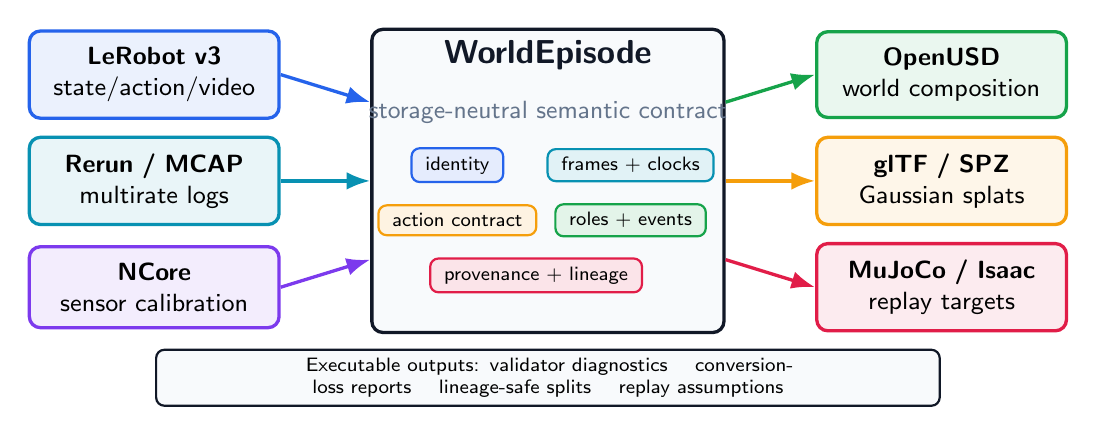
\begin{tikzpicture}[font=\sffamily]
  \node[wecard=weBlue, text width=2.75cm, minimum height=1.0cm] (lerobot) at (0,1.8) {\textbf{LeRobot v3}\\state/action/video};
  \node[wecard=weCyan, text width=2.75cm, minimum height=1.0cm] (rerun) at (0,0.45) {\textbf{Rerun / MCAP}\\multirate logs};
  \node[wecard=weViolet, text width=2.75cm, minimum height=1.0cm] (ncore) at (0,-0.9) {\textbf{NCore}\\sensor calibration};

  \node[wecard=weInk, fill=wePanel, text width=4.05cm, minimum height=3.85cm] (core) at (5.0,0.45) {};
  \node[font=\sffamily\bfseries\large, text=weInk] at (core.north) [yshift=-0.35cm] {WorldEpisode};
  \node[font=\sffamily\small, text=weSlate] at (5.0,1.32) {storage-neutral semantic contract};
  \node[wechip=weBlue] at (3.85,0.65) {identity};
  \node[wechip=weCyan] at (6.05,0.65) {frames + clocks};
  \node[wechip=weAmber] at (3.85,-0.05) {action contract};
  \node[wechip=weGreen] at (6.05,-0.05) {roles + events};
  \node[wechip=weRose] at (4.85,-0.75) {provenance + lineage};

  \node[wecard=weGreen, text width=2.75cm, minimum height=1.0cm] (usd) at (10.0,1.8) {\textbf{OpenUSD}\\world composition};
  \node[wecard=weAmber, text width=2.75cm, minimum height=1.0cm] (gltf) at (10.0,0.45) {\textbf{glTF / SPZ}\\Gaussian splats};
  \node[wecard=weRose, text width=2.75cm, minimum height=1.0cm] (sim) at (10.0,-0.9) {\textbf{MuJoCo / Isaac}\\replay targets};

  \draw[wearrow=weBlue] (lerobot.east) -- ($(core.west)+(0,1.0)$);
  \draw[wearrow=weCyan] (rerun.east) -- (core.west);
  \draw[wearrow=weViolet] (ncore.east) -- ($(core.west)+(0,-1.0)$);
  \draw[wearrow=weGreen] ($(core.east)+(0,1.0)$) -- (usd.west);
  \draw[wearrow=weAmber] (core.east) -- (gltf.west);
  \draw[wearrow=weRose] ($(core.east)+(0,-1.0)$) -- (sim.west);

  \node[wechip=weInk, fill=wePanel, text width=9.6cm, align=center] at (5,-2.05)
    {Executable outputs: validator diagnostics \quad conversion-loss reports \quad lineage-safe splits \quad replay assumptions};
\end{tikzpicture}%
}
\caption{WorldEpisode is the semantic bridge between robot-learning containers, reconstructed
world assets, and simulator targets. It preserves the world--episode contract without replacing
the storage formats on either side.}
\label{fig:worldepisode-bridge}
\end{figure}

The paper's core claim is therefore not a new monolithic file format. It is an executable
interchange profile for world--episode semantics: identity, frames, clocks, action contracts,
representation roles, events, provenance, uncertainty, and lineage-safe evaluation splits. The
current artifact includes a JSON Schema, semantic validator, round-trip binding artifacts, an
active public LeRobotDataset v3 conversion experiment, hand-authored independent fixtures, and
controlled experiments for replay drift, leakage, and counterfactual augmentation.

\section{Problem Statement and Scope}

WorldEpisode binds an episode to a world revision. The base state is:
\begin{equation}
  W_e(t) = W^{(r)} \oplus \Delta W_e(t),
\end{equation}
where \(W^{(r)}\) is an immutable, content-addressed world revision, \(\Delta W_e(t)\) is the
ordered sequence of episode-specific state changes, \(e\) is a robot-learning episode, and \(t\) is
expressed in an explicitly declared clock domain.

An episode is modeled as:
\begin{equation}
E =
\langle
M, W^{(r)}, B, K, F, C, O, A, X, V, P, Q
\rangle ,
\end{equation}
where \(M\) is the manifest, \(B\) the embodiment, \(K\) task/outcome semantics, \(F\) the frame
graph, \(C\) clocks, \(O\) persistent entities and representations, \(A\) action-space contract,
\(X\) synchronized trace, \(V\) world deltas and events, \(P\) provenance, and \(Q\) quality and
uncertainty records.

Version 1 is intentionally narrow: rigid tabletop manipulation with fixed-base single- or dual-arm
robots. Humanoids, locomotion, deformables, fluids, and multi-agent worlds are later profiles. This
keeps conformance executable rather than aspirational.

WorldEpisode reuses existing standards rather than replacing them. USD~\citep{usd} carries composed
simulation worlds, glTF carries Gaussian appearance assets~\citep{gltf_gs}, NCore carries capture
and pose-graph conventions~\citep{ncore}, Rerun carries physical-data recordings with column
chunks~\citep{rerun}, and ROS/MCAP carries logs. WorldEpisode specifies the semantic relationships
those bindings must preserve.

\section{WorldEpisode Architecture}
\label{sec:architecture}

WorldEpisode is implemented as a sidecar blueprint around existing formats. It does not ask a
LeRobot dataset to become a USD scene, or a USD scene to become a policy-training table. Instead,
it records the relationships those containers need in order to agree about the same episode: the
world revision, persistent entities, space/time conventions, action contract, asset roles,
interaction events, provenance, and split lineage.

Figure~\ref{fig:worldepisode-bridge} shows the intended data flow. Dataset and log containers plug
in on the left; world assets and replay targets plug in on the right; the WorldEpisode sidecar
holds the semantics that would otherwise be scattered across undocumented loader assumptions.

\begin{figure}[t]
\centering
\resizebox{\linewidth}{!}{%
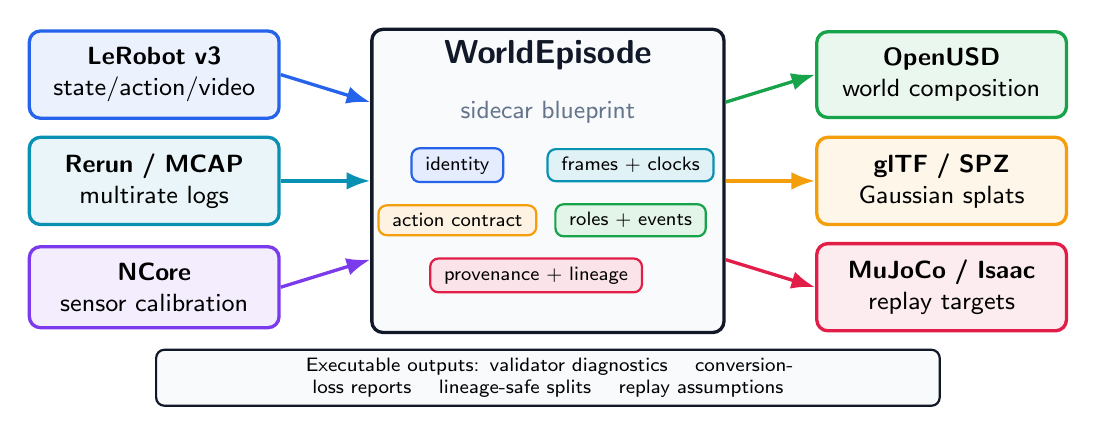
\begin{tikzpicture}[font=\sffamily]
  \node[wecard=weBlue, text width=2.75cm, minimum height=1.0cm] (lerobot) at (0,1.8) {\textbf{LeRobot v3}\\state/action/video};
  \node[wecard=weCyan, text width=2.75cm, minimum height=1.0cm] (rerun) at (0,0.45) {\textbf{Rerun / MCAP}\\multirate logs};
  \node[wecard=weViolet, text width=2.75cm, minimum height=1.0cm] (ncore) at (0,-0.9) {\textbf{NCore}\\sensor calibration};

  \node[wecard=weInk, fill=wePanel, text width=4.05cm, minimum height=3.85cm] (core) at (5.0,0.45) {};
  \node[font=\sffamily\bfseries\large, text=weInk] at (core.north) [yshift=-0.35cm] {WorldEpisode};
  \node[font=\sffamily\small, text=weSlate] at (5.0,1.32) {sidecar blueprint};
  \node[wechip=weBlue] at (3.85,0.65) {identity};
  \node[wechip=weCyan] at (6.05,0.65) {frames + clocks};
  \node[wechip=weAmber] at (3.85,-0.05) {action contract};
  \node[wechip=weGreen] at (6.05,-0.05) {roles + events};
  \node[wechip=weRose] at (4.85,-0.75) {provenance + lineage};

  \node[wecard=weGreen, text width=2.75cm, minimum height=1.0cm] (usd) at (10.0,1.8) {\textbf{OpenUSD}\\world composition};
  \node[wecard=weAmber, text width=2.75cm, minimum height=1.0cm] (gltf) at (10.0,0.45) {\textbf{glTF / SPZ}\\Gaussian splats};
  \node[wecard=weRose, text width=2.75cm, minimum height=1.0cm] (sim) at (10.0,-0.9) {\textbf{MuJoCo / Isaac}\\replay targets};

  \draw[wearrow=weBlue] (lerobot.east) -- ($(core.west)+(0,1.0)$);
  \draw[wearrow=weCyan] (rerun.east) -- (core.west);
  \draw[wearrow=weViolet] (ncore.east) -- ($(core.west)+(0,-1.0)$);
  \draw[wearrow=weGreen] ($(core.east)+(0,1.0)$) -- (usd.west);
  \draw[wearrow=weAmber] (core.east) -- (gltf.west);
  \draw[wearrow=weRose] ($(core.east)+(0,-1.0)$) -- (sim.west);

  \node[wechip=weInk, fill=wePanel, text width=9.6cm, align=center] at (5,-2.05)
    {Executable outputs: validator diagnostics \quad conversion-loss reports \quad lineage-safe splits \quad replay assumptions};
\end{tikzpicture}%
}
\caption{WorldEpisode is the semantic bridge between robot-learning containers, reconstructed
world assets, and simulator targets. It preserves the world--episode contract without replacing
the storage formats on either side.}
\label{fig:worldepisode-bridge}
\end{figure}

This architecture gives the paper its central rule: keep native containers for the data they are
good at storing, but make the cross-container assumptions explicit, checkable, and loss-aware.

\section{The leWorldLayout Format}

The authored document has one primary object, \texttt{world\_layout}, plus optional environment
metadata. Listing~\ref{lst:minimal-layout} shows the minimal shape.

\begin{figure}[t]
\begin{verbatim}
{
  "schema_version": "le-world-layout-0.1",
  "world_layout": {
    "name": "desk-setup",
    "objects": [],
    "scenario_time_ms": 0,
    "scenario_duration_ms": 0,
    "urdf_xml": "<robot name=\"demo\"/>",
    "joint_positions": {},
    "cameras": []
  },
  "environment": {
    "frame_convention": "ros-rep-103"
  }
}
\end{verbatim}
\caption{Minimal \texttt{leWorldLayout} document shape.}
\label{lst:minimal-layout}
\end{figure}

\subsection{Object Model}

Every object records a stable id, pose, dimensions, type, optional semantic role, optional
appearance representations, optional physics geometry, and optional consistency metadata linking
appearance to physics.

World objects are represented with three layers:
\begin{itemize}[leftmargin=*]
  \item \textbf{identity}: \texttt{id}, \texttt{name}, and optional semantic role;
  \item \textbf{layout}: \texttt{type}, \texttt{position\_xyz}, \texttt{rotation\_rpy\_rad},
    \texttt{size\_xyz}, and \texttt{color};
  \item \textbf{transfer}: \texttt{appearance}, \texttt{physics}, and \texttt{consistency}.
\end{itemize}

\subsection{Appearance and Physics}

The central design choice is that appearance does not imply collision. The \texttt{appearance}
layer stores render and perception representations such as primitives, meshes, and Gaussian splats.
The \texttt{physics} layer stores collision geometry, mass, inertia, friction, restitution, and
fixed/collision flags. The \texttt{consistency} layer records how the two correspond, for example
a hand-authored collider, bounding-box fit, convex decomposition, or unchecked import.

\subsection{Portable Asset References}

Every asset reference must be a portable relative path. References may not include URI schemes,
absolute paths, empty path segments, or \texttt{.}/\texttt{..} traversal. This rule is what lets a
layout travel as a folder or registry artifact without rewriting paths for each machine.

\subsection{Boundary With Scenarios}

A layout is not a task. A scenario references a layout and adds task instruction, role bindings,
randomization, policy and control timing, success conditions, guards, and evaluation metrics. This
separation lets the same world support inspection, editing, simulator transfer, dataset packaging,
and benchmark execution.


\section{Reference Implementation}

URDF Studio provides the initial reference implementation. It validates the current World format,
imports layouts from JSON files, folders, or links, resolves portable asset references, and
transfers static layouts into multiple downstream targets.

The relevant implementation components are:
\begin{itemize}[leftmargin=*]
  \item schema and validator generation from typed backend models;
  \item browser import/export for world JSON and folders with assets;
  \item static transfer services for simulator workspaces;
  \item asset-reference validation shared by frontend and backend paths;
  \item cross-simulator transfer into MuJoCo, Genesis, PyBullet, MJX/MJLab, and Blender;
  \item scenario-level benchmark execution above the layout layer.
\end{itemize}

The reference implementation is an existence proof, not a dependency requirement. The proposed norm
is the data contract: other tools should be able to emit and validate the same documents without
depending on URDF Studio.


\section{Conformance and Evaluation}

WorldEpisode should be evaluated as an executable standard, not only as a schema.

\paragraph{RQ1: semantic preservation across bindings.}
Convert the same dataset through LeRobot, WorldEpisode, Rerun, NCore, MCAP, OpenUSD, and glTF
Gaussian assets. Measure field retention, semantic retention, deterministic round-trip equality,
externalized fields, approximated fields, and declared loss.

\paragraph{RQ2: physical-coherence fault detection.}
Inject controlled failures: wrong transform direction, millimeters interpreted as meters,
quaternion-order mismatch, timestamp offset, stale calibration, action frame mislabeled, collision
mesh scale mismatch, reused entity id, or world revision changed without a new hash. Measure
validator precision, recall, and diagnosis quality.

\paragraph{RQ3: cross-simulator replay.}
Replay the same demonstrations in at least two simulators. Measure end-effector RMSE, object
trajectory RMSE, grasp-state agreement, contact-event precision/recall/F1, final-state pose error,
task-outcome agreement, and success-rate rank correlation across policy checkpoints.

\paragraph{RQ4: downstream robustness.}
Train with observations/actions alone, with unstructured 3D side files, and with full WorldEpisode
identity/world alignment. Evaluate shifted camera extrinsics, unseen viewpoints, object displacement,
background replacement, distractors, occlusion, lighting changes, novel object instances, and held-out
worlds.

\paragraph{RQ5: lineage-safe splits.}
Compare random episode splits against task-, world-, entity-, and reconstruction-lineage-disjoint
splits. A substantial performance drop under lineage-safe splits would show that current dataset
abstractions overestimate generalization.

The minimum credible reference release should include a small golden conformance corpus: valid
minimal packages, valid advanced packages, intentionally invalid packages, lossy-conversion examples,
and cross-simulator replay fixtures.

\section{Limitations and Open Gates}
\label{sec:limits}

The current evidence is deliberately scoped. It is meant to expose hidden failure mechanisms, not
to claim full robot-learning, game-engine, or autonomous-driving generality.

Table~\ref{tab:evidence-boundaries} states the boundary of each empirical claim. This is important
because the paper argues for a semantic contract, not for a finished benchmark suite.

\begin{table}[htbp]
\centering
\footnotesize
\caption{What the current evidence supports, and what it does not yet support.}
\label{tab:evidence-boundaries}
\begin{tabular}{@{}>{\raggedright\arraybackslash}p{0.19\linewidth}
                >{\raggedright\arraybackslash}p{0.43\linewidth}
                >{\raggedright\arraybackslash}p{0.32\linewidth}@{}}
\toprule
Claim area & Current evidence & Boundary \\
\midrule
Leakage & Public ArmnetBench LeRobot audit with 400 teleoperated reference episodes, an executable
Torch BC probe, a measured temporal ridge state/action baseline, an ACT/Diffusion gate harness, and
four compact digest-verified LeRobot state/action split packages totaling 241{,}470 frames &
Stronger ACT/Diffusion jobs are prepared but not run; the compact split packages omit video
payloads, so no vision-policy, real-robot, or high-fidelity rollout result is claimed yet \\
Conversion & Two pinned public LeRobotDataset v3 five-episode batch round trips with exact tensor,
index, and timestamp equality & Two datasets; broader LeRobot coverage remains future work \\
Replay timing & Real SO-101 trajectory alignment, tested same-trace MuJoCo and Genesis
position-servo replay adapters, URDF Studio MuJoCo/Genesis episode-backend evidence, and a
dependency-free scheduler conformance harness & One LeRobot trace with minimal joint replay
adapters; no contact-rich task rollout, Isaac runtime result, or SAPIEN runtime result is claimed \\
Meta-simulator neutrality & Adapter contract matrix over MuJoCo, Isaac Sim, Genesis, and SAPIEN
plus same-trace MuJoCo/Genesis replay evidence, URDF Studio \texttt{SimBackend} conformance, and a
one-episode MuJoCo--Genesis comparison & MuJoCo and Genesis are tested for the minimal replay
profile; Isaac and SAPIEN are not replay-tested in this paper, and equal physics is not claimed \\
Generalization beyond robotics & Deterministic game-engine collision-patch and autonomous-driving
clock-domain pilots using the same invariant vocabulary & Not measured on production game engines,
public AV datasets, or fleet logs \\
Validation & Fourteen injected requirement faults, two independent hand-authored fixtures, and a
pilot natural-source corpus over five public datasets & Five-dataset count is met through active
LeRobot artifacts plus source-level public benchmark metadata; dataset-specific diagnostic reports
now cover all cases, but no maintainer feedback is recorded yet \\
Binding retention & Versioned \texttt{uss-core-23} semantic projection checked by executable
artifacts & Pilot projection; not a universal score of each storage format \\
Famous benchmark call-out & Source-level audit over Open X-Embodiment, DROID, BridgeData V2,
LIBERO, and CALVIN, plus a targeted DROID subset rerun tool and a separate inflation-proof gate &
Missing public controls are not measured score inflation; the proof gate currently has one
executed DROID subset rerun, zero inflation-proof famous-benchmark rerun reports, and zero measured
inflation claims \\
Real-to-sim drift & Controlled action-contract and representation-role ablations where drifted
contracts succeed in simulation and fail under deployment proxies & Deterministic proxy; not a
RoboSnap/DROID-Sim rerun or physical hardware deployment \\
Adoption & Public schema, installable local preflight package, validator, fixtures, governance
files, and an internal clean-room reader that does not import the reference SDK & No PyPI release,
upstream LeRobot/Rerun integration, external independent implementation, or external dataset release
yet \\
Scale architecture & Dataset manifest schema, scalable example, executable audit, and a generated
32{,}768-shard catalog benchmark describing 1{,}073{,}741{,}824 episodes for open/index latency,
partition pruning, digest-cache behavior, and resolver routing & Catalog-side benchmark only; no
billion episode rows, payload bytes, distributed storage, concurrent readers, or institutional
federation are measured \\
\bottomrule
\end{tabular}
\end{table}

\FloatBarrier

\begin{openresult}{results not claimed in this release}
The artifact keeps unfinished claims executable instead of hiding them. The current RFC release gate
is:
\texttt{python3 tools/release\_readiness.py --strict-rfc}. The full-standard gate is:
\texttt{python3 tools/release\_readiness.py --strict-full}. The latter is expected to fail until
the two gates boxed below are backed by committed reports and, additionally, external standard
evidence exists: maintainer-reviewed diagnostics, an independently written reader/exporter, and at
least one externally published WorldEpisode-compatible dataset. The same gates are indexed in
\path{docs/experiments/open_reproduction_gates/open_reproduction_gates.json}.
\end{openresult}

\begin{openresult}{ACT/Diffusion and rollout impact}
Status: open (referenced from Case 1). To close this gate, first regenerate the split packages and
LeRobot job specs with \texttt{python3 tools/lerobot\_policy\_leakage\_gate.py}. Then run the
generated jobs with \texttt{bash docs/experiments/lerobot\_policy\_gate/run\_lerobot\_policy\_jobs.sh}
inside a LeRobot training environment.

Required artifacts: policy checkpoint digests, train/eval configs and seeds, offline action
metrics for random and scene-disjoint splits, rollout traces or videos with content digests, and an
updated \path{docs/experiments/lerobot_policy_gate/policy_gate_report.json}.

Acceptance rule: at least one ACT or Diffusion Policy run must report both split protocols, and at
least one simulator or physical rollout report must use the same split manifest. Until then, the
paper claims only the offline Torch probe and the prepared gate.
\end{openresult}

\begin{openresult}{famous-benchmark score-inflation proof}
Status: open (referenced from Case 7). A targeted DROID subset rerun can be attempted with
\texttt{uv run --with pyarrow --with requests --with numpy python
tools/famous\_benchmark\_policy\_rerun.py --benchmark droid\_100 --required}. The proof contract is
then enforced with \texttt{python3 tools/benchmark\_inflation\_gate.py --required}.

Required artifacts: benchmark-specific WorldEpisode conversion, lineage/timing audit, faithful
published-protocol policy rerun, paired corrected evaluation under the same metric, and a measured
baseline-minus-corrected score drop.

Acceptance rule: the gate must contain at least one inflation-proof valid rerun report with
\texttt{measured\_inflation=true}. Source-level metadata gaps alone are evidence of missing
controls, not evidence that published scores are inflated.
\end{openresult}

\paragraph{Beyond robotics (future work).}
All measured evidence in this paper is the WorldEpisode robotics profile; the broader Universal
Spatial State framing is proposed, not demonstrated outside robotics. Two deterministic pilots only
illustrate that the same vocabulary can express non-robotics drift. In a game-engine collision pilot,
a client loads a stale arena collision asset after an authoritative patch, which the asset-digest,
state-revision, and role checks catch. In an autonomous-driving clock pilot, camera and lidar logs
deserialize correctly, but a 50 ms undeclared clock offset at 15 m/s creates a 0.75 m fusion error
against a 0.20 m tolerance, which the declared clock mapping corrects to 0.0 m. These are
illustrative pilots, not production game-engine or AV benchmark results. A stronger paper should add
at least one public non-robotics corpus and an independently maintained adapter.\collabmark{C6}

\paragraph{The two weakest links, stated plainly.}
First, the leakage result is an offline behavioral-cloning audit, not a physical rollout: the Torch
MLP probe and the temporal ridge baseline demonstrate that random splits can leak world lineage and
inflate offline evaluation, but ACT and Diffusion Policy must be run on the committed split
manifest (and the split packages' source videos mirrored with digests) before claiming impact on
common LeRobot training recipes. Second, the reference implementation is single-sourced: the
clean-room reader reduces the risk that the fixtures only work through the reference SDK, but it is
an internal artifact, and the \texttt{worldepisode} package is not yet a released PyPI package or
merged into upstream LeRobot or Rerun examples. The pilot natural-source corpus adds 19 cases from
five public robot-learning datasets but does not prove prevalence in the wild; a stronger version
of this paper should record whether dataset maintainers agree with representative
diagnostics.\collabmark{C4}

\section{Discussion}

\paragraph{Not another monolithic binary.}
WorldEpisode should have a small semantic core and multiple bindings. LeRobot can be the
policy-training view; Rerun the multirate physical-data view; NCore the sensor/reconstruction
capture view; MCAP/ROS the raw log view; OpenUSD/SimReady the composed simulation-world view; glTF
or SPZ the Gaussian asset view; and a reference directory the conformance profile.

\paragraph{Lineage-safe evaluation.}
Episode-level random splits can leak the same reconstructed room, physical object, Gaussian asset,
source video, world revision, or generated asset lineage across training and evaluation.
WorldEpisode should support split constraints such as \texttt{world\_lineage},
\texttt{physical\_entity}, \texttt{source\_capture}, \texttt{reconstruction\_run}, and
\texttt{generated\_asset\_family}.

\paragraph{Standards alignment.}
The project should align with standards bodies rather than antagonize them. Static 3D robot-map
exchange, humanoid dataset lifecycle, OpenLABEL annotation, glTF Gaussian splats, USD composition,
and NCore capture conventions are all useful neighbors. WorldEpisode is an executable profile and
bridge across those layers.

\paragraph{Reviewer red team.}
Likely criticisms are predictable: ``this is just USD,'' ``GSDF already combines splats and
physics,'' ``Rerun already solves robot data,'' or ``a schema is not research.'' The response is to
ship adapters, conformance fixtures, fault-injection evaluation, replay metrics, and lineage-split
evidence rather than relying on schema novelty alone.

\section{Conclusion}
\label{sec:conclusion}

Robot-learning failures often arrive disguised as clean data: valid tensors, valid videos, valid
scene files, and invalid state assumptions. WorldEpisode makes those
assumptions explicit. It binds interaction data to immutable state revisions, gives persistent
identity to entities, declares space/time/transition semantics, assigns roles to assets, records
events and provenance, and reports conversion loss instead of hiding it.

In the reference experiments, a random split overlaps every task--scene proxy lineage; a
task-confounded holdout increases mean episode nRMSE from \ExpMlpRandomNrmse{} to
\ExpMlpHeldoutNrmse{} for the MLP and from \ExpTemporalRandomNrmse{} to
\ExpTemporalHeldoutNrmse{} for deterministic temporal ridge. This diagnoses an invalid random split
but does not isolate scene leakage. Freezing a \ExpTimingDelayFrames-frame telemetry lag on
\ExpTimingCalibrationEpisodes{} calibration trajectories reduces pooled RMSE from
\ExpTimingZeroRmse{} to \ExpTimingFrozenRmse{} over \ExpTimingHeldoutEpisodes{} held-out
trajectories. This does not measure motor-effective latency. The validator catches every injected
fault class. A preregistered \ExpContactReplayScenarioCount-scenario MuJoCo/Genesis contact audit
reaches \ExpContactReplayFOne{} contact F1 and complete task-outcome agreement while exposing
\ExpContactReplayFinalOrientationDeg$^\circ$ final-orientation disagreement. The contribution is
the auditable contract and its failure boundaries, not a claim of physical rollout improvement or
equivalent physics.

The next experiments must disentangle task from physical scene lineage, run ACT/Diffusion and
rollouts over matched seeds, instrument command and motor-effective timestamps on another controller,
and anchor articulated contact replay to hardware observations. Until then, the paper makes no
famous-benchmark inflation, simulator-independent physics, or mature-standard claim.


\bibliographystyle{plainnat}
\bibliography{references}

\end{document}
